\documentclass[3p,preprint,12pt]{elsarticle}

\journal{}

\usepackage{tabulary,xcolor}
\usepackage{amsfonts,amsmath,amssymb}
\usepackage[normalem]{ulem}
\usepackage{enumitem}
\usepackage[T1]{fontenc}

\usepackage{url,multirow,morefloats,floatflt,cancel}

\usepackage{makecell}

\usepackage{colortbl}
\usepackage{xcolor}
\usepackage{pifont}
\usepackage[nointegrals]{wasysym}
\usepackage{floatrow}
\usepackage{pgfplots,algorithmic,algorithm}
\pgfplotsset{compat=newest}
\usepackage{textgreek}
% \usetikzlibrary{external}
% \tikzexternalize[prefix=tikz/]

\usepackage{booktabs}

%\usepackage[finalizecache]{minted}
%\usepackage[frozencache]{minted}
\usepackage{minted}

\usepackage[toc,page]{appendix}
\usepackage{bm}

\usepackage{pifont}
\newcommand{\cmark}{\ding{51}}
\newcommand{\xmark}{\ding{55}}

\usepackage{graphicx,amssymb,amsmath,amsthm}

\newcommand{\mP}{\mathcal{P}}

\newcommand{\bx}{{x}}
\newcommand{\bX}{{X}}

\newcommand{\by}{{y}}
\newcommand{\bt}{\bm{\theta}}
\newcommand{\bc}{{c}}
\newcommand{\bw}{{w}}
\newcommand{\bxi}{{\xi}}
\newcommand{\bbeta}{{\eta}}

\newcommand{\bz}{{z}}
\newcommand{\bzero}{{0}}
\renewcommand{\bf}{{f}}
\newcommand{\bu}{{u}}

\newcommand{\RR}{\mathbb{R}}
\newcommand{\bv}{{v}}
\usepackage{calc}
\usepackage{accents}
\newcommand{\dbtilde}[1]{\accentset{\approx}{#1}}
\newcommand{\vardbtilde}[1]{\hat{\raisebox{0pt}[0.85\height]{$\hat{#1}$}}}

\usepackage{booktabs,bm,float}
\usepackage{tcolorbox}

%\usepackage[noend]{algpseudocode}

\usepackage{hyperref}
\usepackage[nameinlink]{cleveref}

\newtheorem{definition}{Definition}
\newtheorem{remark}{Remark}

\Crefname{equation}{eq.}{eqns.}
\Crefname{equation}{Eq.}{Eqns.}

% \usepackage{autonum}

\usepackage{subcaption}

\newcommand{\rev}[1]{{\color{blue}#1}}
\usepackage{makecell}
\begin{document}
\newtheorem{theorem}{Theorem}
\newtheorem{lemma}{Lemma}

%\usepackage{pifont}% http://ctan.org/pkg/pifont
%\newcommand{\cmark}{\ding{51}}%
%\newcommand{\xmark}{\ding{55}}%
\begin{frontmatter}

\title{}

\author[]{}
\ead{}
\address[]{}
 

%\todo[inline]{you need to fix the biblio; lots of errors.}
%
%\todo[inline]{fix all errors with articles; you are missing them in several places}
%
%\todo[inline]{I feel you should spend more time thinking about the structure and organization of the document; you often explain things without a clear or logical order; for each section/subsection your goal should be to explain a series of points; then you should lay out a logical order to introduce the concepts. Once the structure is clear you can start writing.}
 
\begin{abstract}
\end{abstract}

\begin{keyword}

\end{keyword}

\end{frontmatter}


\section{Introduction}


\section{Automatic Differentiation}


\section{AD in Scientific Machine Learning}


\section{Applications of AD in Physical Applications}

Traditionally, applications of automatic differentiation in machine learning and scientific computing are largely isolated. In machine learning, AD has been popularized by deep learning, where AD is used to compute gradients of deep neural networks. In scientific computing, AD has a long history for calculating adjoints of numerical PDE schemes. 

Nowadays, AD are being customized to leverage heterogeneous computing environments (e.g., multiprocessing and distributed computing) and serve physics informed machine learning, where physical models are mixed with machine learning models. 

In this section, we present three applications that reflect current practice of applying AD to physical simulations. Specifically, in the first example, we show how we implement an ODE solver with an AD framework; in the second example, we show how we can improve performance critical parts in an AD framework with specialized numerical algorithms  using custom operators; in the third example, we show how we combine numerical PDE solvers with deep neural networks and non-machine learning models. 

We use ADCME, which is an automatic differentiation library built on TensorFlow, for implementing the numerical benchmarks. ADCME extends the capabilities of TensorFlow to numerical simulations by providing or enhancing many missing features, such as sparse linear algebra, MPI operations, numerical PDE schemes, etc. 


\subsection{Lorenz System}

The Lorenz system is a simplified mathematical model for atmospheric convection

\begin{equation}
    \begin{aligned}
    \frac{d x}{dt} &= \sigma (y-x)\\
    \frac{d y}{dt} &= x(\rho - z) - y\\
    \frac{d z}{dt} &= xy - \beta z\\
    \end{aligned}
\end{equation}
Here $x$, $y$, and $z$ correspond to the rate of convection, the horizontal temperature variation, and the vertical temperature variation, respectively. $(\sigma, \rho, \beta)$ are the parameters, which can be learned by solving the constrained optimization problem 

\begin{equation}\label{equ:rv-disc}
    \begin{aligned}
    \min_{\sigma, \rho, \beta} &\; \sum_{i=1}^n (x_i - \hat x_i)^2 + (y_i - \hat y_i)^2 + (z_i - \hat z_i)^2 \\ 
    \text{s.t.} &\; (x_{i+1}, y_{i+1}, z_{i+1}) = \mathbf{F}(x_i, y_i, z_i; \sigma, \rho, \beta) \quad i = 0, 1, \ldots, n-1
    \end{aligned}
\end{equation}
Here $\hat x_i$, $\hat y_i$, and $\hat z_i$ are observations at time step $i$ and $\mathbf{F}$ is a time integrator. Note that \cref{equ:rv-disc} can be easily extended to sparse observations, i.e., only part of $\{\hat x_i, \hat y_i, \hat z_i\}$ are observable, by changing the objective function. 

In the experiment, the initial condition is given by $x_0 = 1, y_0= 0, z_0 = 0$, and the ODE is solved with a fourth-order explicit Runge–Kutta temporal integrator with time-step $\Delta t = 0.03$. The following code shows how we can implement the ODE solver with ADCME

\begin{minted}{julia}
function runge_kutta_one_step(f::Function, t::PyObject, y::PyObject, Δt::PyObject, θ::Union{PyObject, Missing})
    k1 = Δt*f(t, y, θ)
    k2 = Δt*f(t+Δt/2, y+k1/2, θ)
    k3 = Δt*f(t+Δt/2, y+k2/2, θ)
    k4 = Δt*f(t+Δt, y+k3, θ)
    y = y + k1/6 + k2/3 + k3/3 + k4/6
end

function rk4(f::Function, T::Union{PyObject, Float64}, 
                NT::Union{PyObject,Int64}, y::Union{PyObject, Float64, Array{Float64}}, θ::Union{PyObject, Missing}=missing)
    one_step = runge_kutta_one_step
    
    ta = TensorArray(NT+1) # storing y
    function condition(i, ta)
        i <= NT+1
    end
    function body(i, ta)
        y = read(ta, i-1)
        y_ = one_step(f, (cast(eltype(Δt), i)-1)*Δt, y, Δt, θ)
        ta = write(ta, i, y_)
        i+1, ta 
    end
    ta = write(ta, 1, y)
    i = constant(2, dtype=Int32)
    _, out = while_loop(condition, body, [i, ta])
    res = stack(out)
end
\end{minted}
The function \texttt{runge\_kutta\_one\_step} is similar to how we typically implement an ODE solver; the only difference is that we need some boiler plates to do loops using an AD language, as in \texttt{rk4}. \texttt{rk4} is already in ADCME, and we can actually solve \Cref{equ:rv-disc} with a few lines of code
\begin{minted}{julia}
using ADCME
using JLD2 

function f(t, y, θ)
    [θ[1]*(y[2]-y[1]);y[1]*(θ[2]-y[3])-y[2];y[1]*y[2]-θ[3]*y[3]]
end
x0 = [1.;0.;0.]
θ = Variable([8.0;30.0;3.0])
solution = rk4(f, 3.0, 100, x0, θ)

@load "lorentz.dat" observations
loss = sum((solution - observations)^2)
sess = Session(); init(sess)

BFGS!(sess, loss, method = "LBFGS")
\end{minted}
The last line wraps gradient calculations and an L-BFGS-B optimizer; for users, solving the constrained optimization problem is essentially a one-line consolidation. 

\begin{figure}
    \centering
    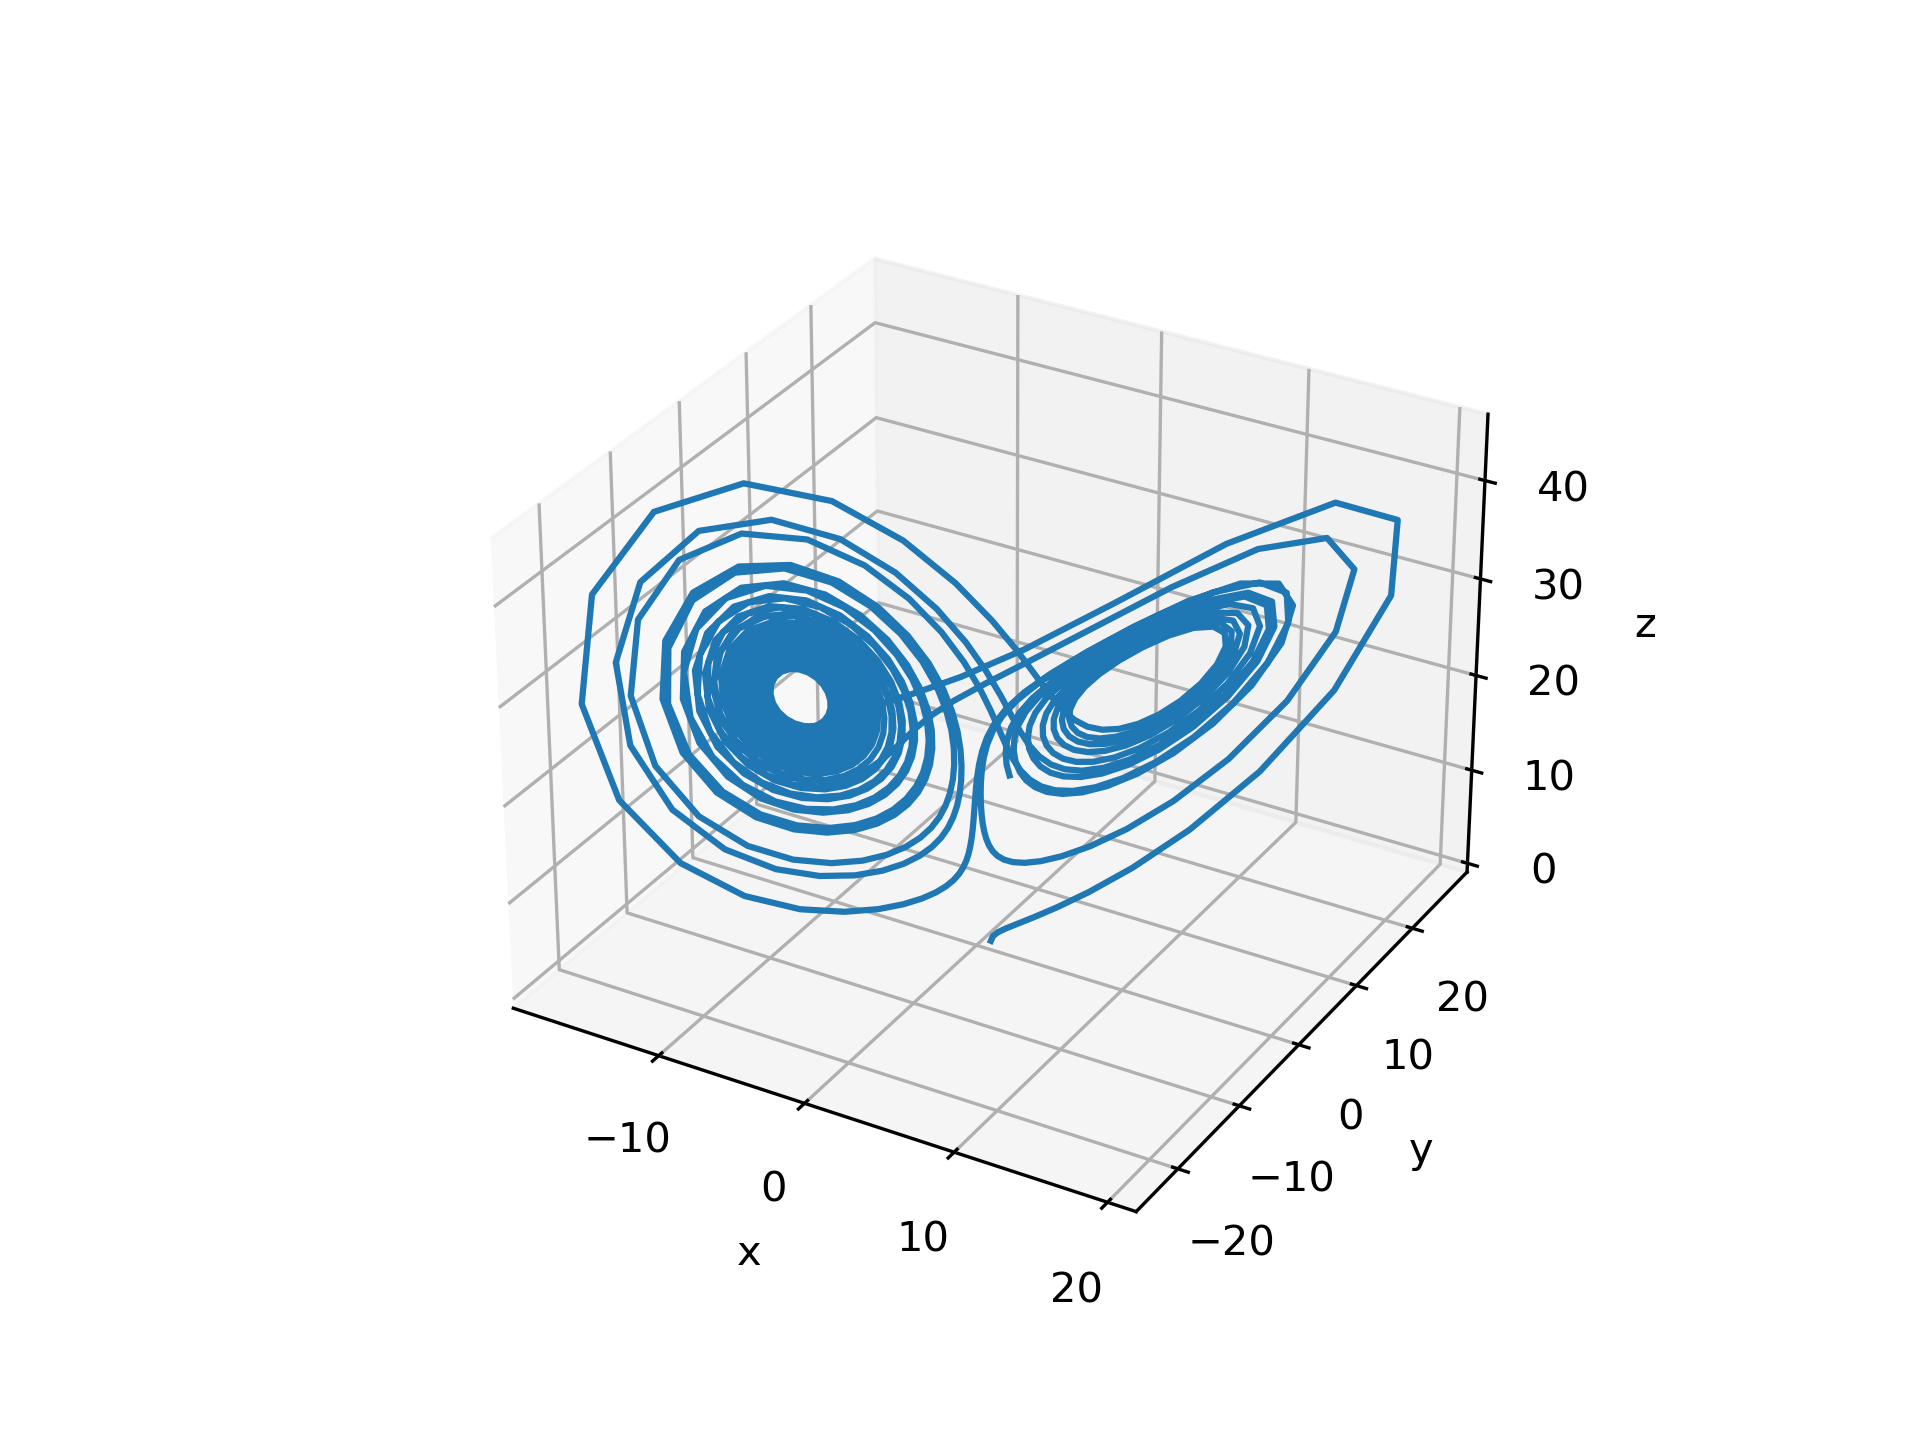
\includegraphics[width=0.59\textwidth]{paper/Kailai/figures/lorentz.png}~
    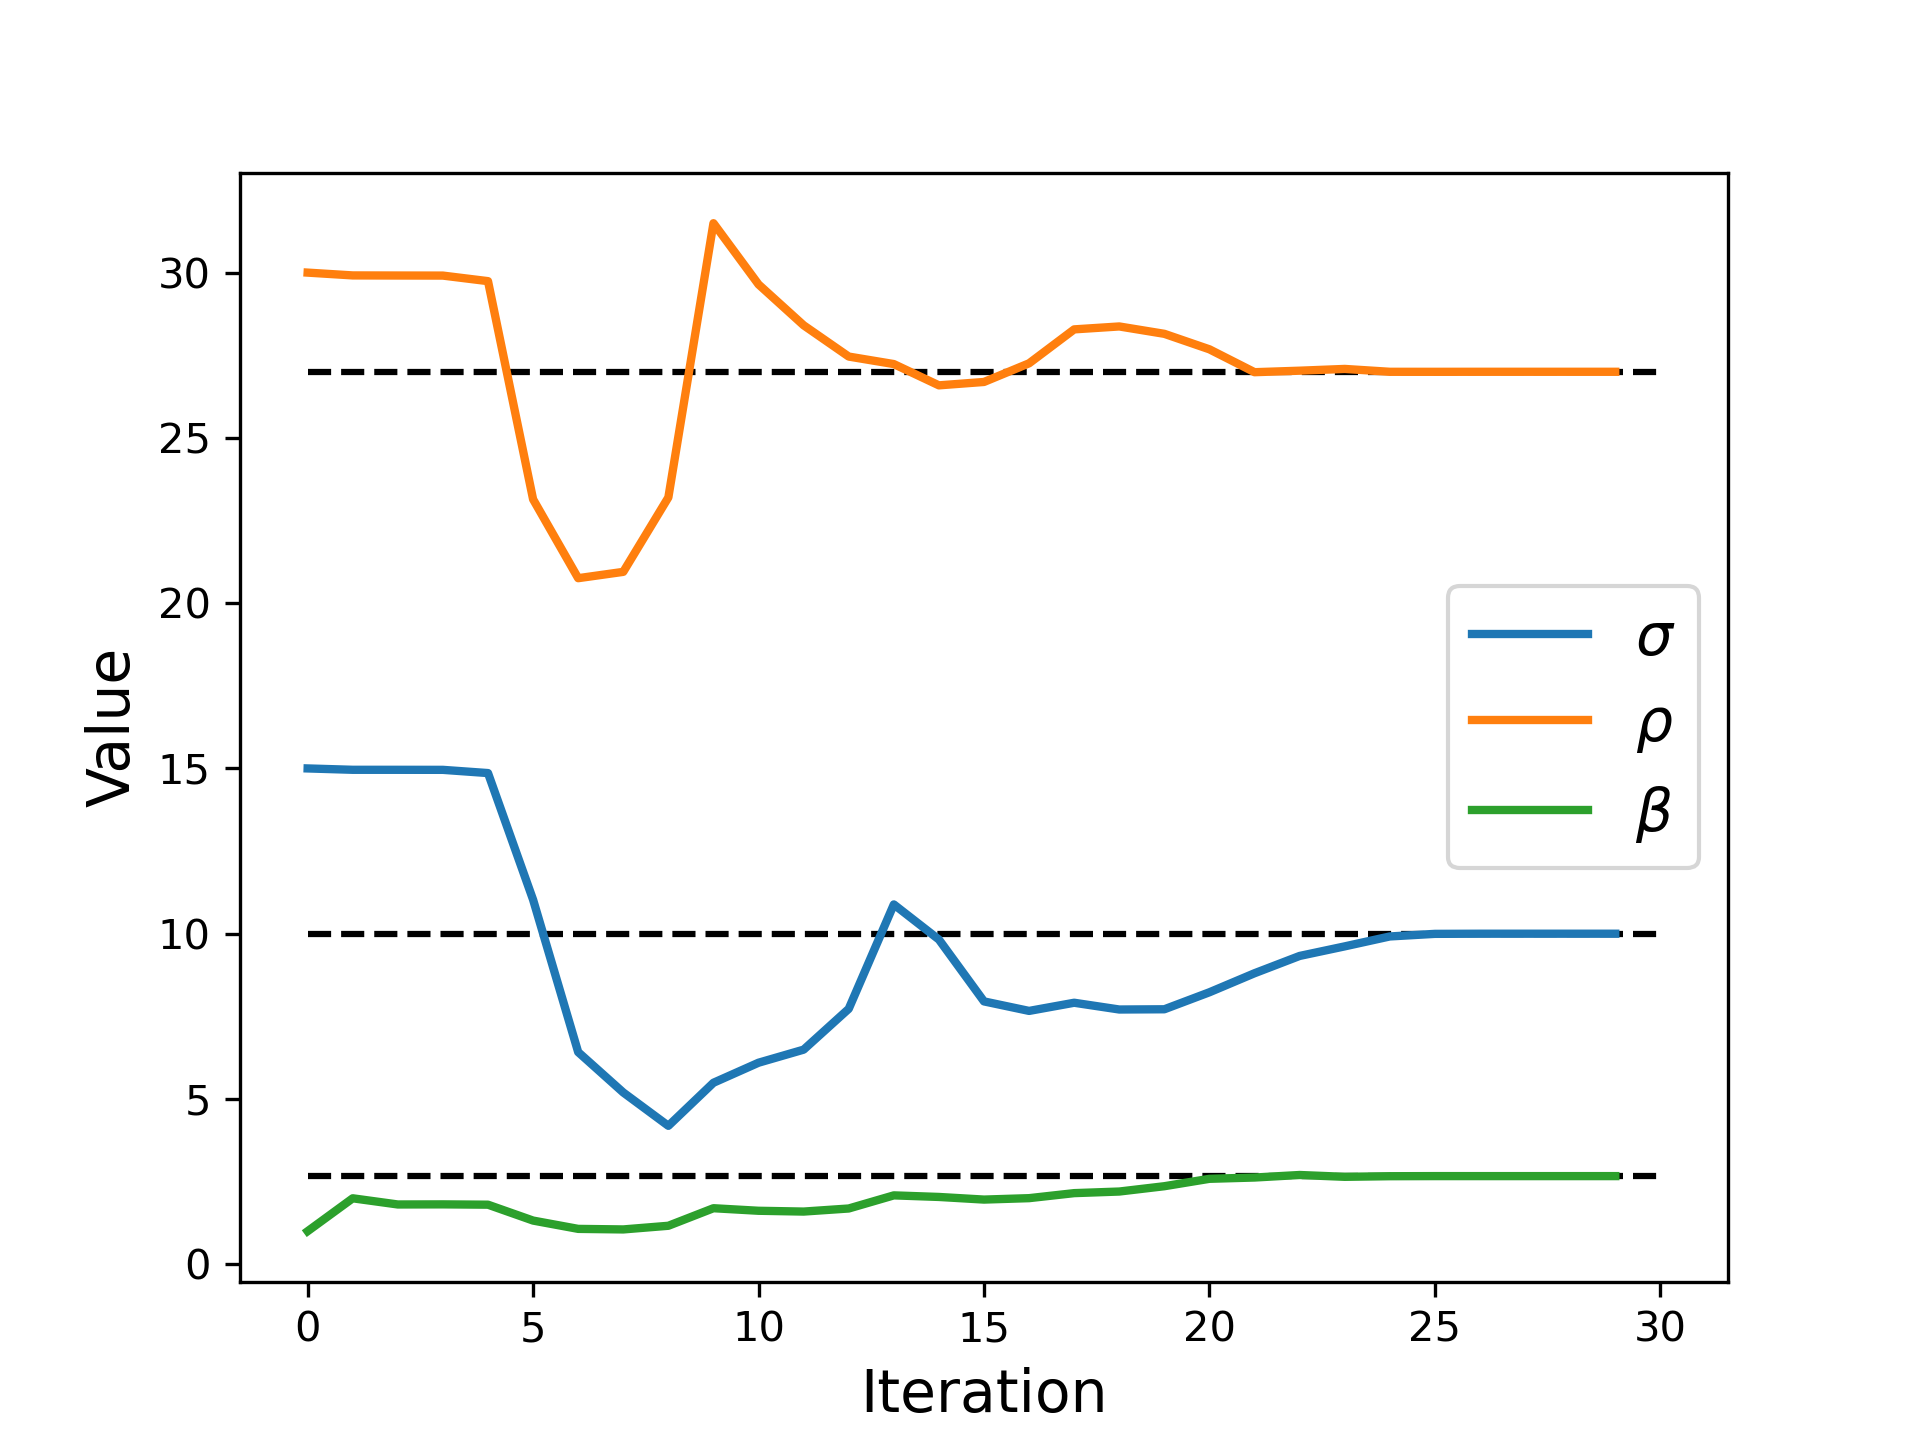
\includegraphics[width=0.39\textwidth]{paper/Kailai/figures/lorentz_converge.png}
    \caption{Caption}
    \label{fig:rv-lorentz}
\end{figure}

The results are summarized in \Cref{fig:rv-lorentz}. In the left panel, we present ground truth solution (observations) with a time horizon $T=30$. The exact parameters are given by 
$$\sigma = 10, \rho = \frac{8}{3}, \beta = 27$$
The right panel shows the convergence of estimated parameters to the ground truth. Despite large differences between initial guess and ground truth, the parameters converge quickly to the ground truth, with only dozens of iterations. 

\subsection{Thomas Algorithm}

Our next example involves designing a custom operator for accelerating solving tridiagonal matrix systems. A tridiagonal matrix system is given by a linear equation of the following form
\begin{equation}\label{equ:software-triproblem}
    \begin{bmatrix}
   {b_1} & {c_1} & {   } & {   } & { 0 } \\
   {a_2} & {b_2} & {c_2} & {   } & {   } \\
   {   } & {a_3} & {b_3} & \ddots & {   } \\
   {   } & {   } & \ddots & \ddots & {c_{n-1}}\\
   { 0 } & {   } & {   } & {a_n} & {b_n}\\
\end{bmatrix}
\begin{bmatrix}
   {x_1 }  \\
   {x_2 }  \\
   {x_3 }  \\
   \vdots   \\
   {x_n }  \\
\end{bmatrix}
=
\begin{bmatrix}
   {d_1 }  \\
   {d_2 }  \\
   {d_3 }  \\
   \vdots   \\
   {d_n }  \\
\end{bmatrix}
\end{equation}
Tridiagonal matrices arise in many physical applications, such as a 3-point finite difference for 1D Poisson's equation. In numerical analysis, a triagonal matrix system can be efficiently solved with the Thomas algorithm. Thomas algorithm is an iterative algorithm and involves many in-place operations. Consequently, it can be quite awkward to implement with an AD framework. Additionally, the gradient calculation procedure generated by AD is also iterative, while more efficient algorithms, such as physics constrained learning, exist for this type of calculations. 

A common practice to leverage ``non-standard'' algorithms is to use custom operators---also known as \textbf{external function support}---in AD. Custom operators require us to implement forward and backward calculations and ``plug'' this operator into the computational graph. 

As an example, the forward computation can be implemented as follows
\begin{minted}{julia}
void TriSolve_forward(double *X, const double *A, 
    const double *b, const double *C, const double *d,
    int n){
    double *B = new double[n]; 
    double *D = new double[n]; 
    memcpy(B, b, sizeof(double)*n);
    memcpy(D, d, sizeof(double)*n);
    for (int i=1;i<n;i++){
        double w = A[i-1]/B[i-1];
        B[i] = B[i] - w * C[i-1];
        D[i] = D[i] - w * D[i-1];
    }
    X[n-1] = D[n-1]/B[n-1];
    for (int i = n-2; i>-1; i--){
        X[i] = (D[i]-C[i]*X[i+1])/B[i];
    }
    delete [] B;
    delete [] D;
}
\end{minted}
and the gradient back-propagation can be implemented as follows
\begin{minted}{julia}
void TriSolve_backward(
    double *grad_A, double *grad_B, double *grad_C, double *grad_D,
    const double *grad_X,
    const double *X, const double *A, 
    const double *B, const double *C, const double *D,
    int n){
    TriSolve_forward(grad_D, C, B, A, grad_X, n);  
    for(int i = 0; i<n; i++){
        if(i>0) grad_A[i-1] = -grad_D[i] * X[i-1];
        grad_B[i] = -grad_D[i] * X[i];
        if(i<n-1) grad_C[i] = -grad_D[i] * X[i+1];
    }
}
\end{minted}

\begin{figure}[htpb]
    \centering
    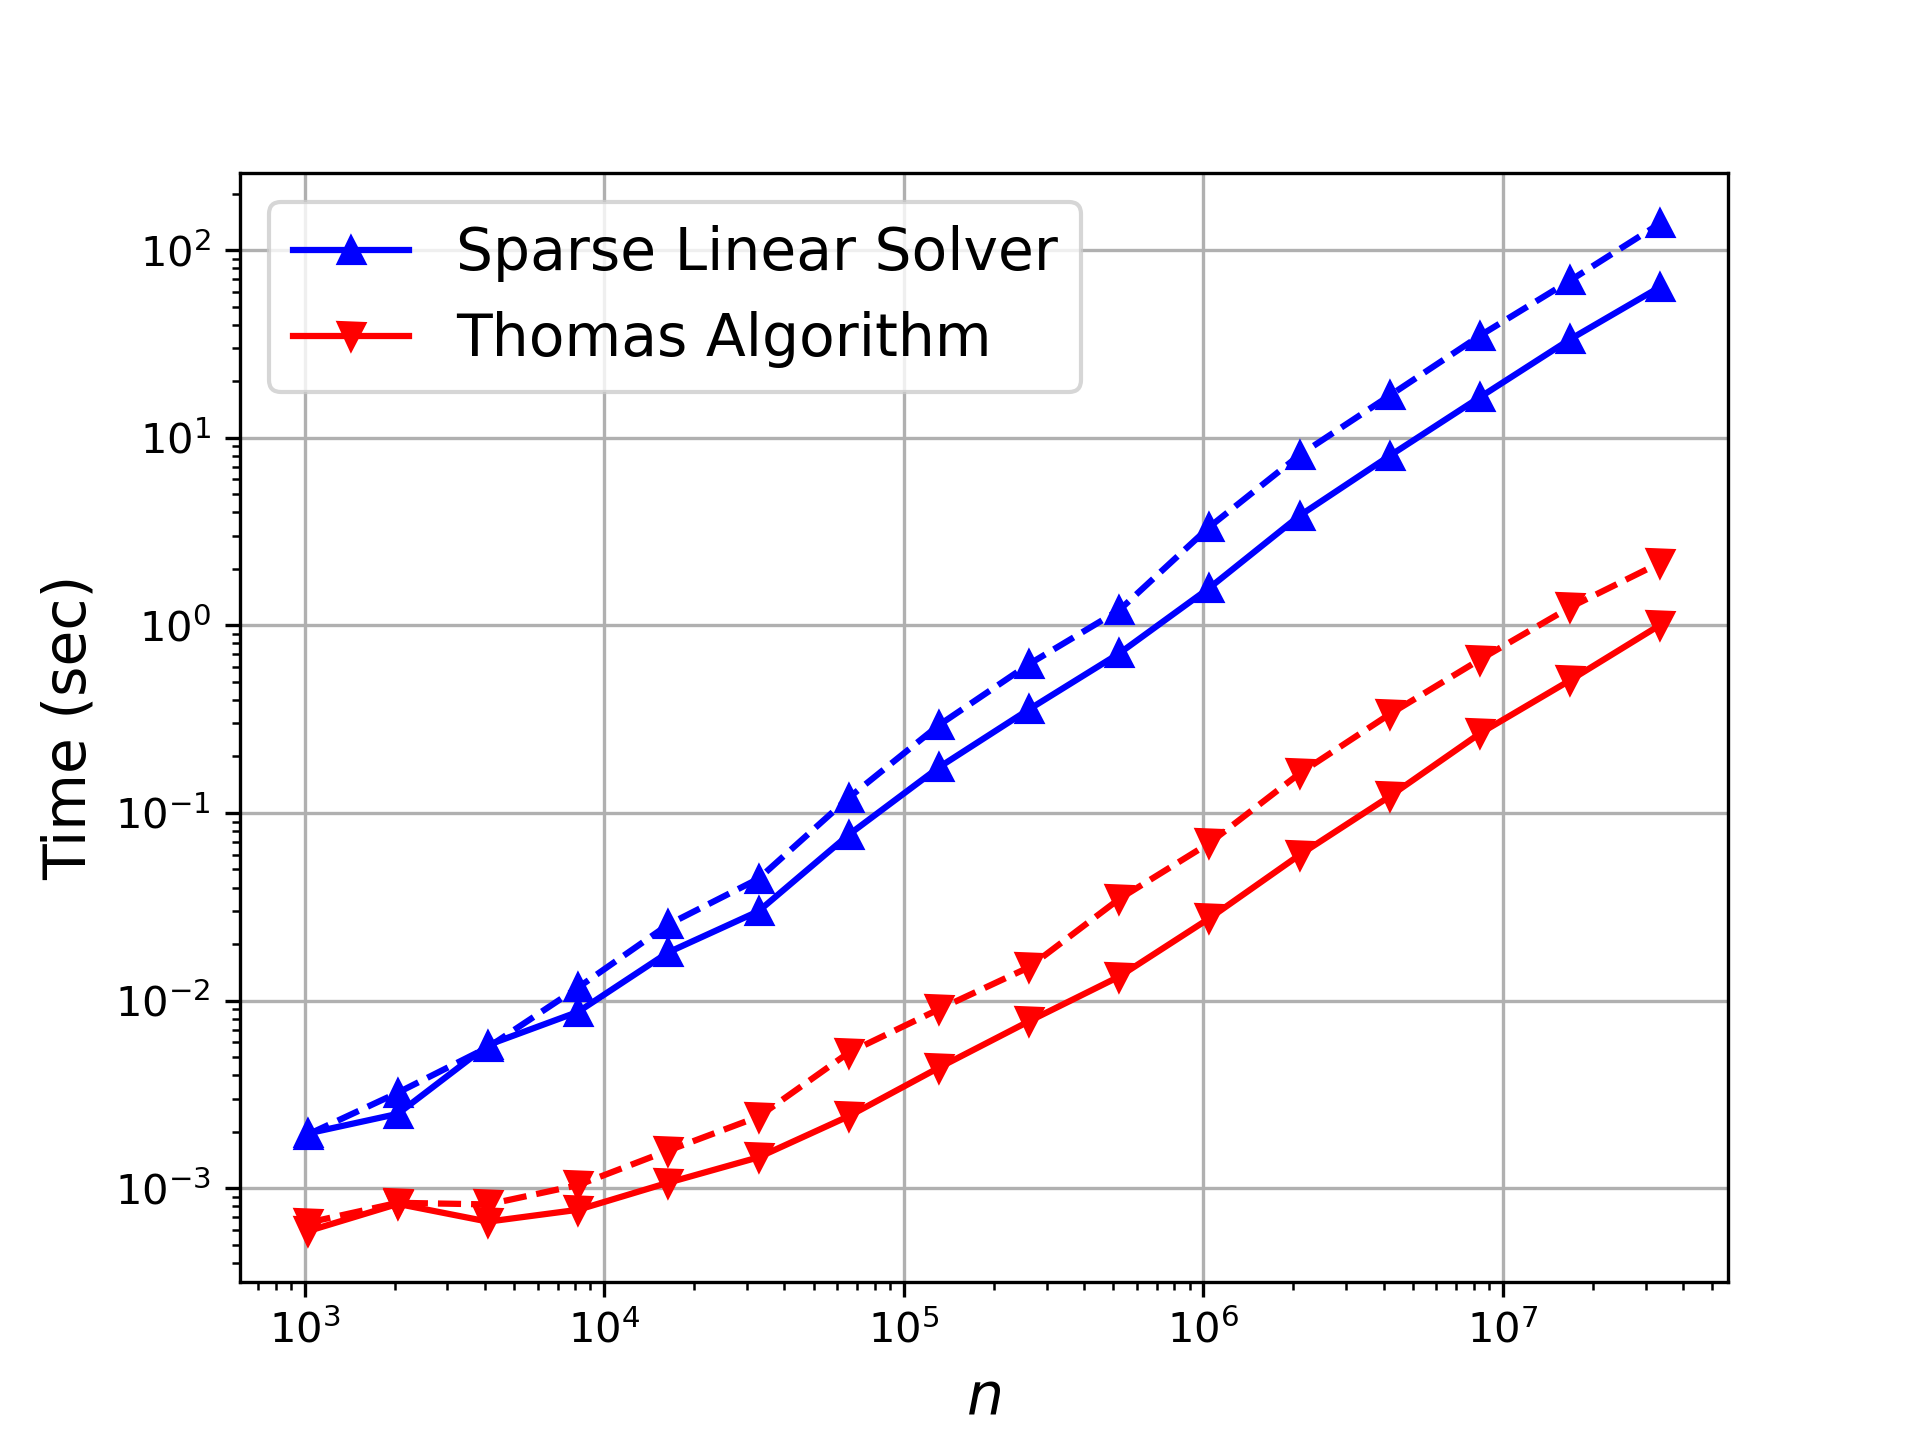
\includegraphics[width=0.8\textwidth]{paper/Kailai/figures/trisolve.png}
    \caption{}
    \label{fig:trisolve}
\end{figure}

The results are shown in \Cref{fig:trisolve}. We compare the performance of the Thomas algorithm with a general-purpose sparse linear solver, sparseLU. It is worth noticing that both algorithms achieve linear scaling, but the Thomas algorithm is around 100 times faster. 

\subsection{Combining PDE Solvers and (non-)Machine Learning Models}

Our last example shows how to combine a numerical PDE solver with a machine learning model, i.e., deep neural networks, or a non-machine learning model, i.e., radial basis function. Consider a Poisson's equation with an unknown diffusivity coefficient
\begin{equation}\label{equ:poisson}
\begin{aligned}
     \nabla \cdot (\kappa(x,y) \nabla u)) &= f(x) & (x,y)\in \Omega\\ 
     u &= 0 & (x,y)\in  \partial\Omega
\end{aligned}
\end{equation}
The training data are given by observations of $u$. \Cref{fig:cforward} shows the solution on a finite element grid. The exact $\kappa$ is given by 
$$\kappa(x,y) = \sin(2\pi x) + y + 2$$
To learn $\kappa$ function, we can approximate $\kappa$ with a deep neural network or a radial basis function
$$\kappa(x,y) \approx \text{N}_\theta(x, y), \quad \kappa(x,y) \approx \sum_{i=1}^n c_i \sqrt{1+(x-x_i)^2 + (y-y_i)^2} + d_0 + d_1 x + d_2 y$$
Here $\text{N}_\theta$ is a deep neural network with the weights and biases $\theta$. In the radial basis function approach, $c_i, d_i$ are trainable parameters, and $(x_i, y_i)$ are predetermined centers.

\begin{figure}[htpb]
    \centering
    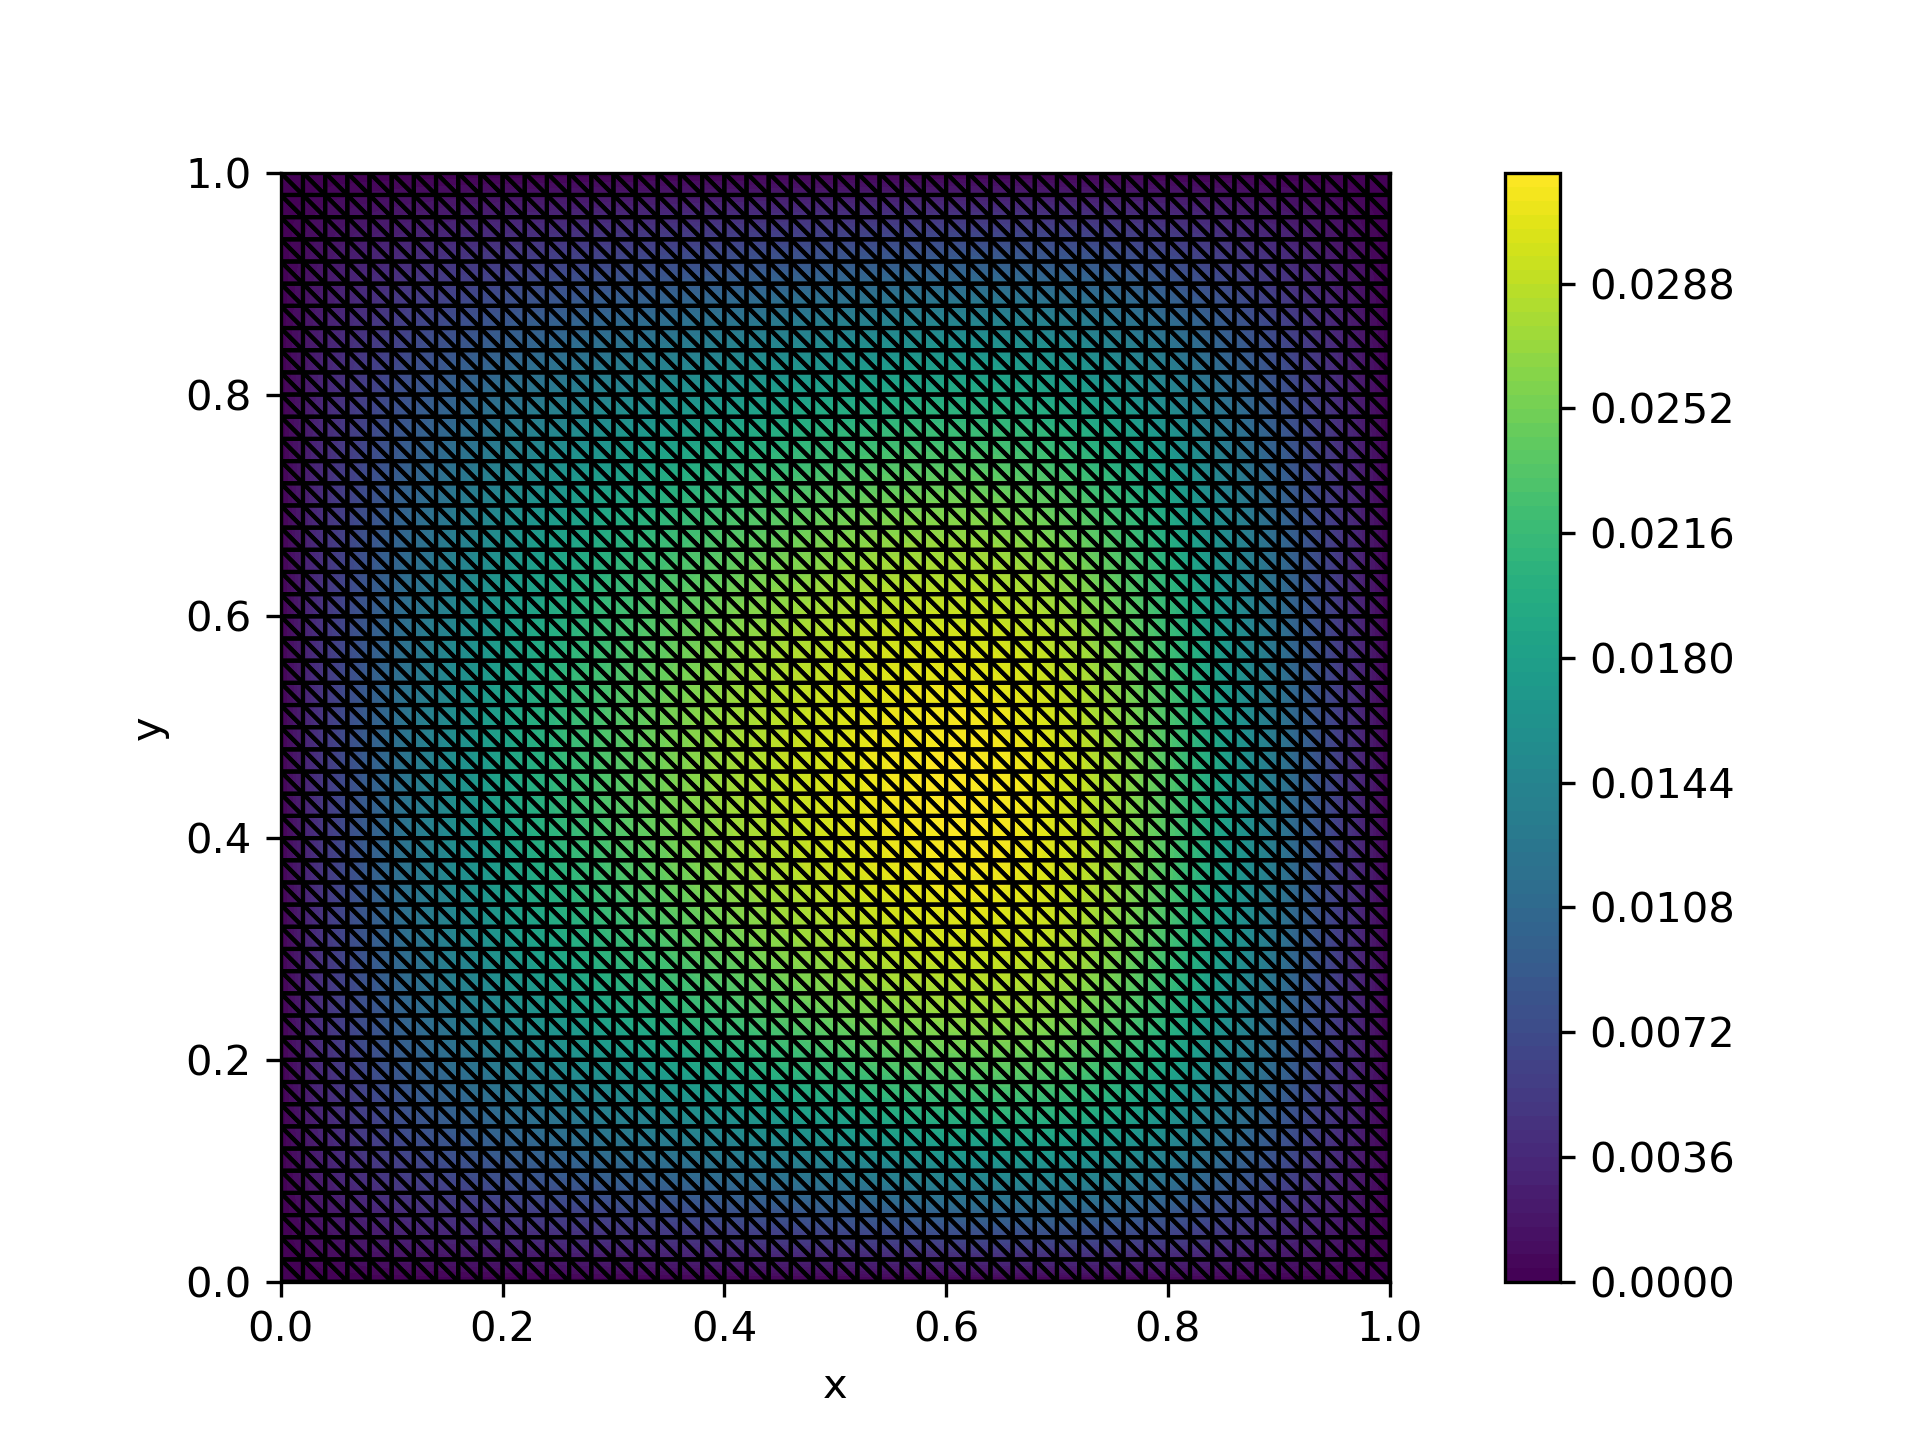
\includegraphics[width=0.8\textwidth]{paper/Kailai/figures/combine_forward.png}
    \caption{}
    \label{fig:cforward}
\end{figure}

In an AD framework, we can easily combining the function approximator of $\kappa$ with a finite element solver for \Cref{equ:poisson} by expressing numerical solvers with computational graphs. The process is rendered almost trivial using AdFem, a computational graph based finite element library built on ADCME. For example, the following code solves the numerical PDE with a deep neural network with 3 hidden layers, 20 neurons per layer, and \texttt{tanh} activation functions. We use $|\text{N}_\theta(x, y) + 3|$ to shift the initial guess away from 0 and ensure that $\kappa$ is always positive. 
\begin{minted}{julia}
using AdFem

f = (x,y)->1.0
mmesh = Mesh(50,50,1/50)
xy = gauss_nodes(mmesh)
κ = abs(squeeze(fc(xy, [20,20,20,1])) + 3.0)
A = compute_fem_laplace_matrix1(κ, mmesh)
F0 = eval_f_on_gauss_pts(f, mmesh)
F = compute_fem_source_term1(F0, mmesh)
bdnode = bcnode(mmesh)
A, F = impose_Dirichlet_boundary_conditions(A, F, bdnode, zeros(length(bdnode)))
sol = A\F 
\end{minted}
Note that the neural network output $\kappa$ can be directly fed to a numerical PDE solver. In gradient back-propagation, the gradients are back-propagated from numerical solvers to deep neural networks. 

\begin{figure}[htpb]
    \centering
    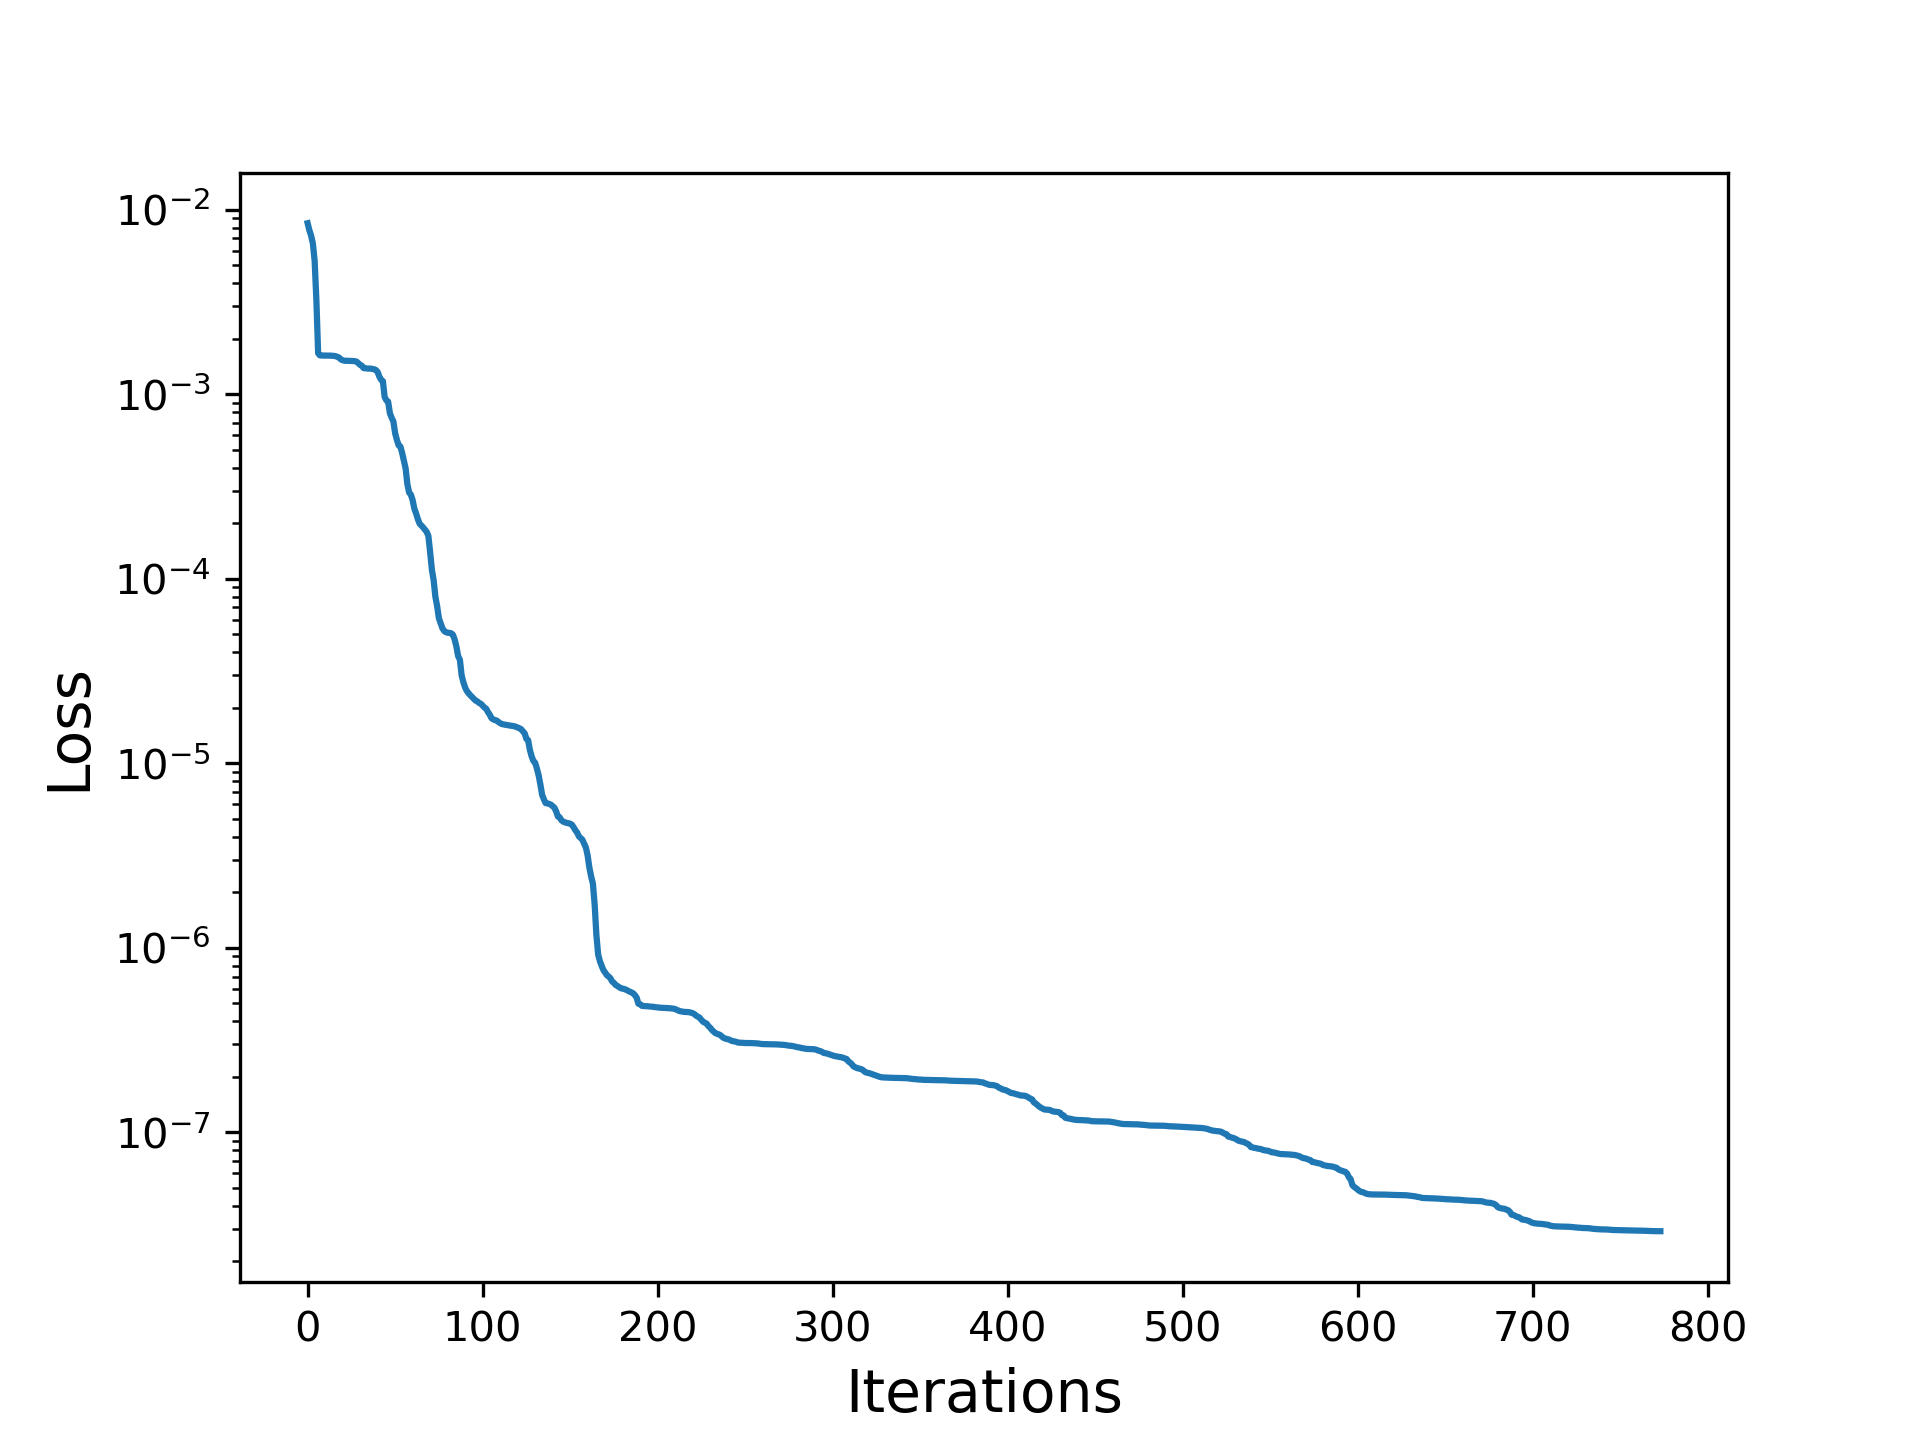
\includegraphics[width=0.49\textwidth]{paper/Kailai/figures/combine_loss.png}~
    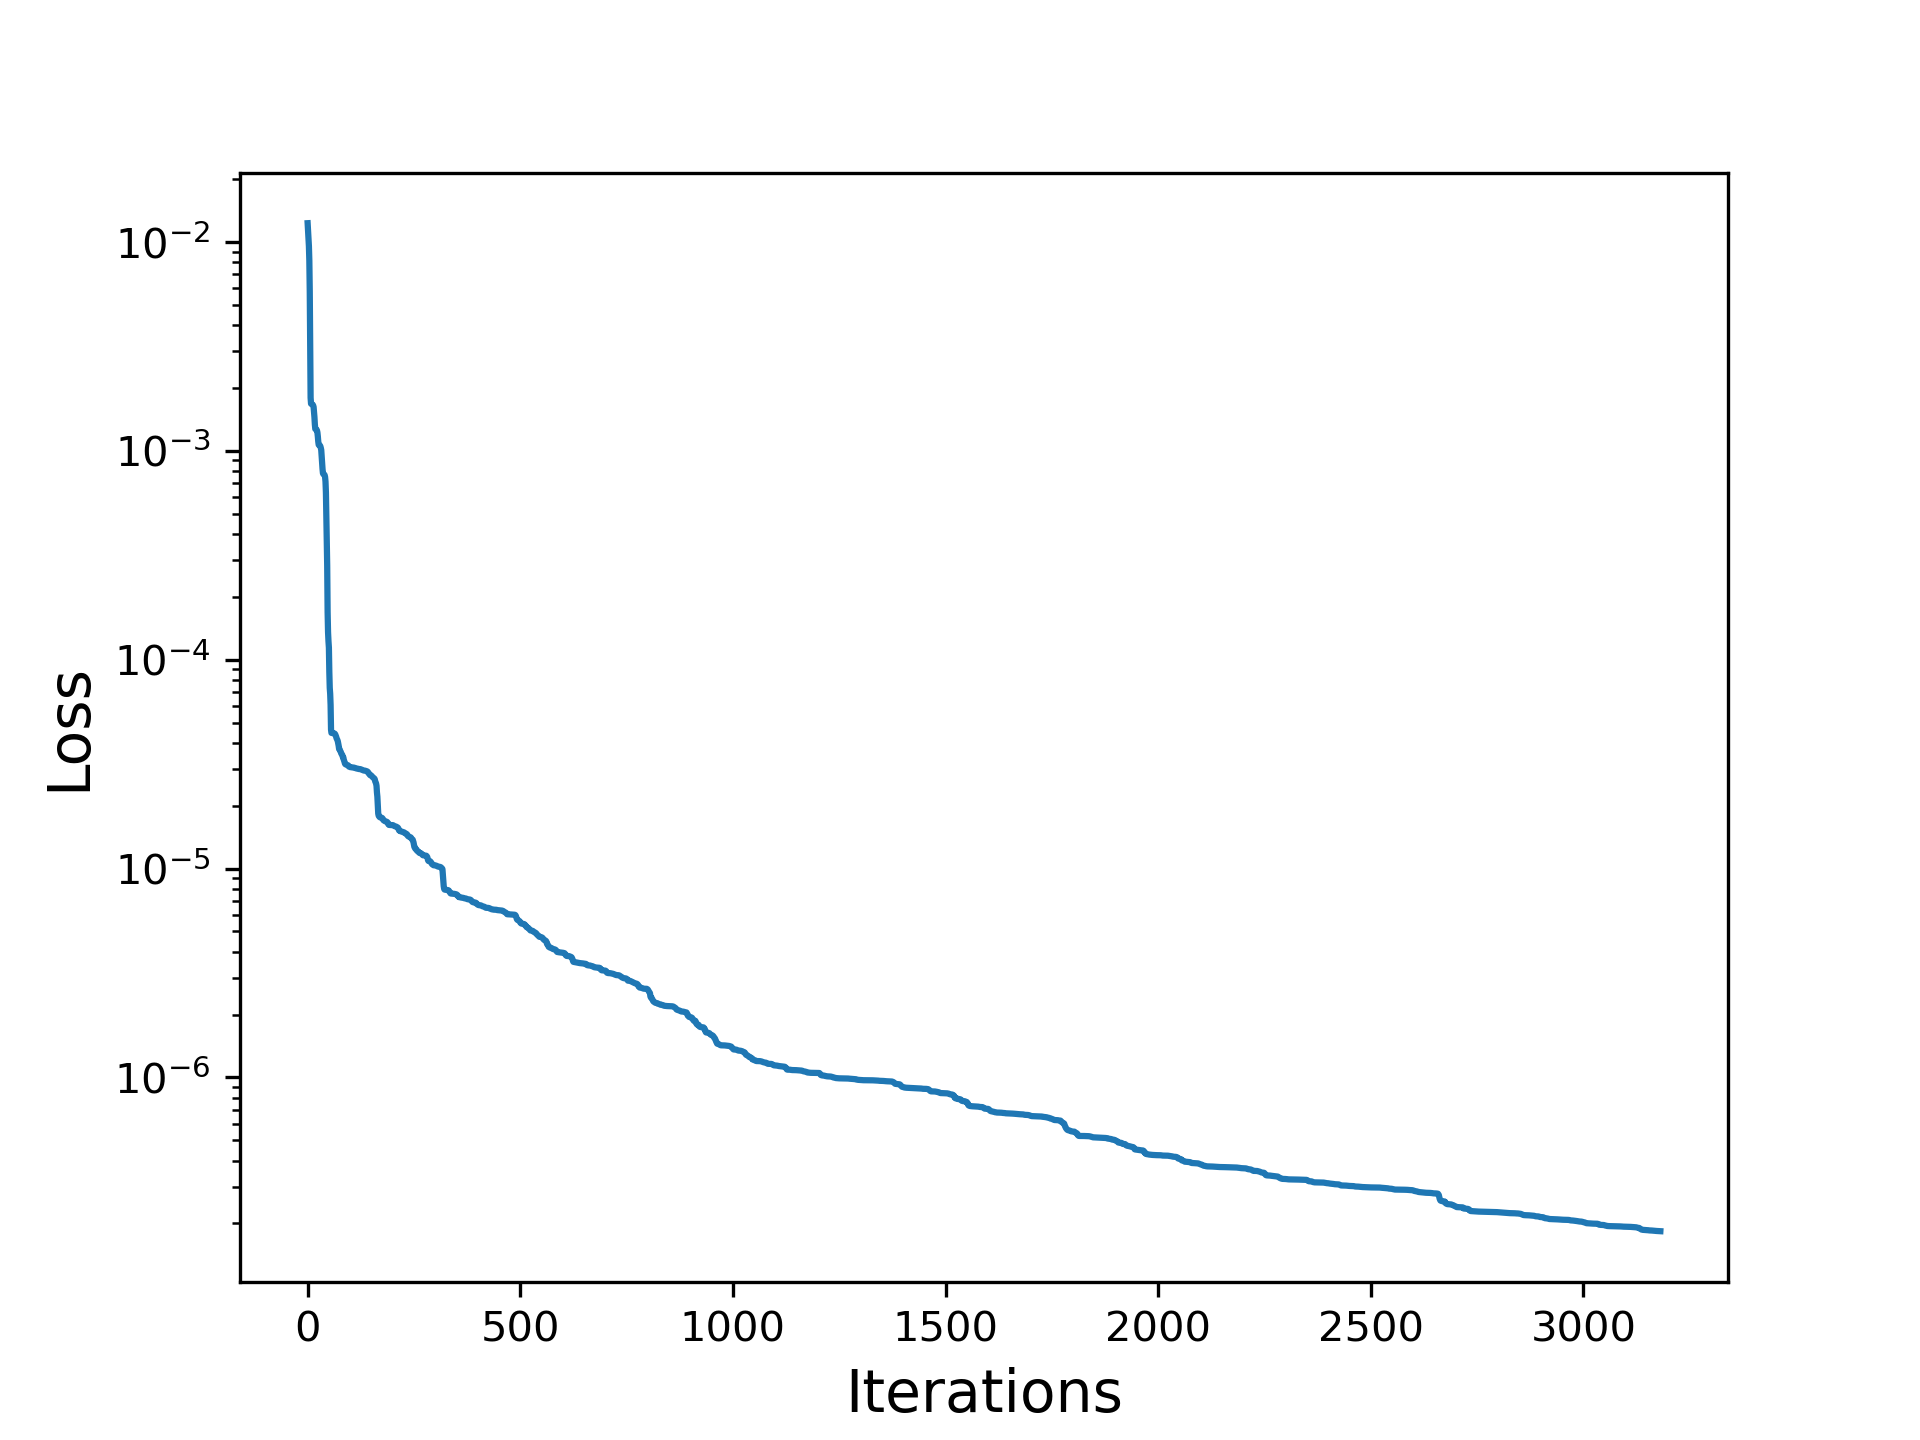
\includegraphics[width=0.49\textwidth]{paper/Kailai/figures/combine_loss_rbf.png}
    \caption{}
    \label{fig:closs_nn}
\end{figure}

\begin{figure}[htpb]
    \centering
    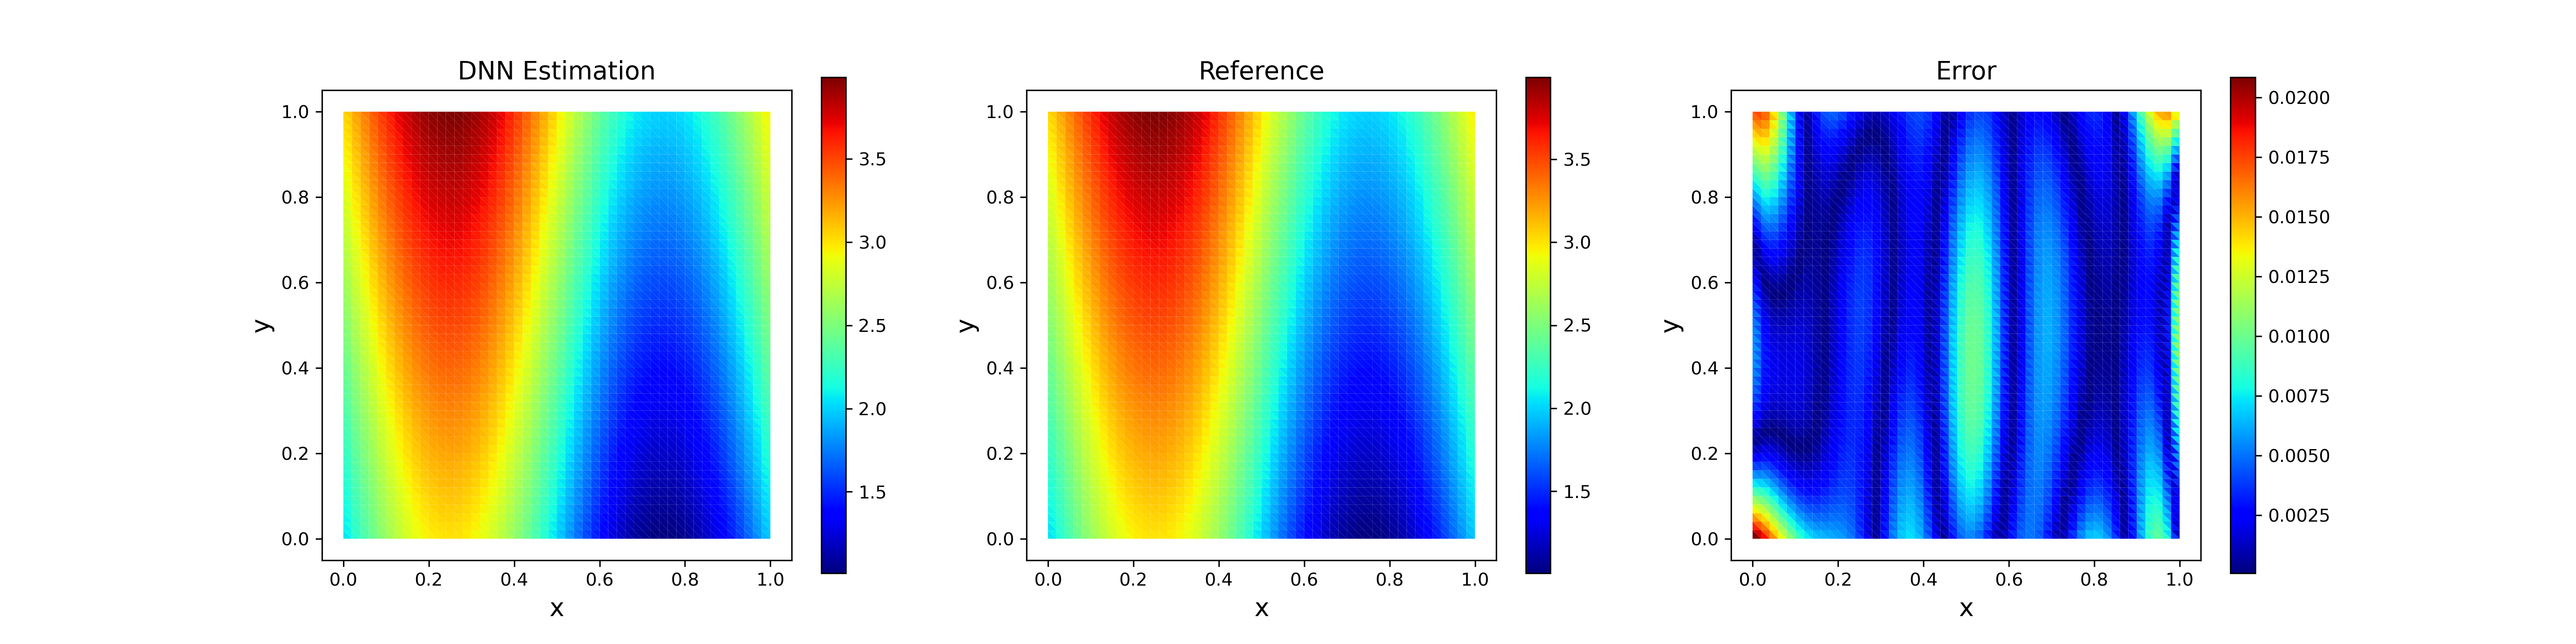
\includegraphics[width=1.0\textwidth]{paper/Kailai/figures/combine_nn.png}
    \caption{}
    \label{fig:nn}
\end{figure}

\begin{figure}[htpb]
    \centering
    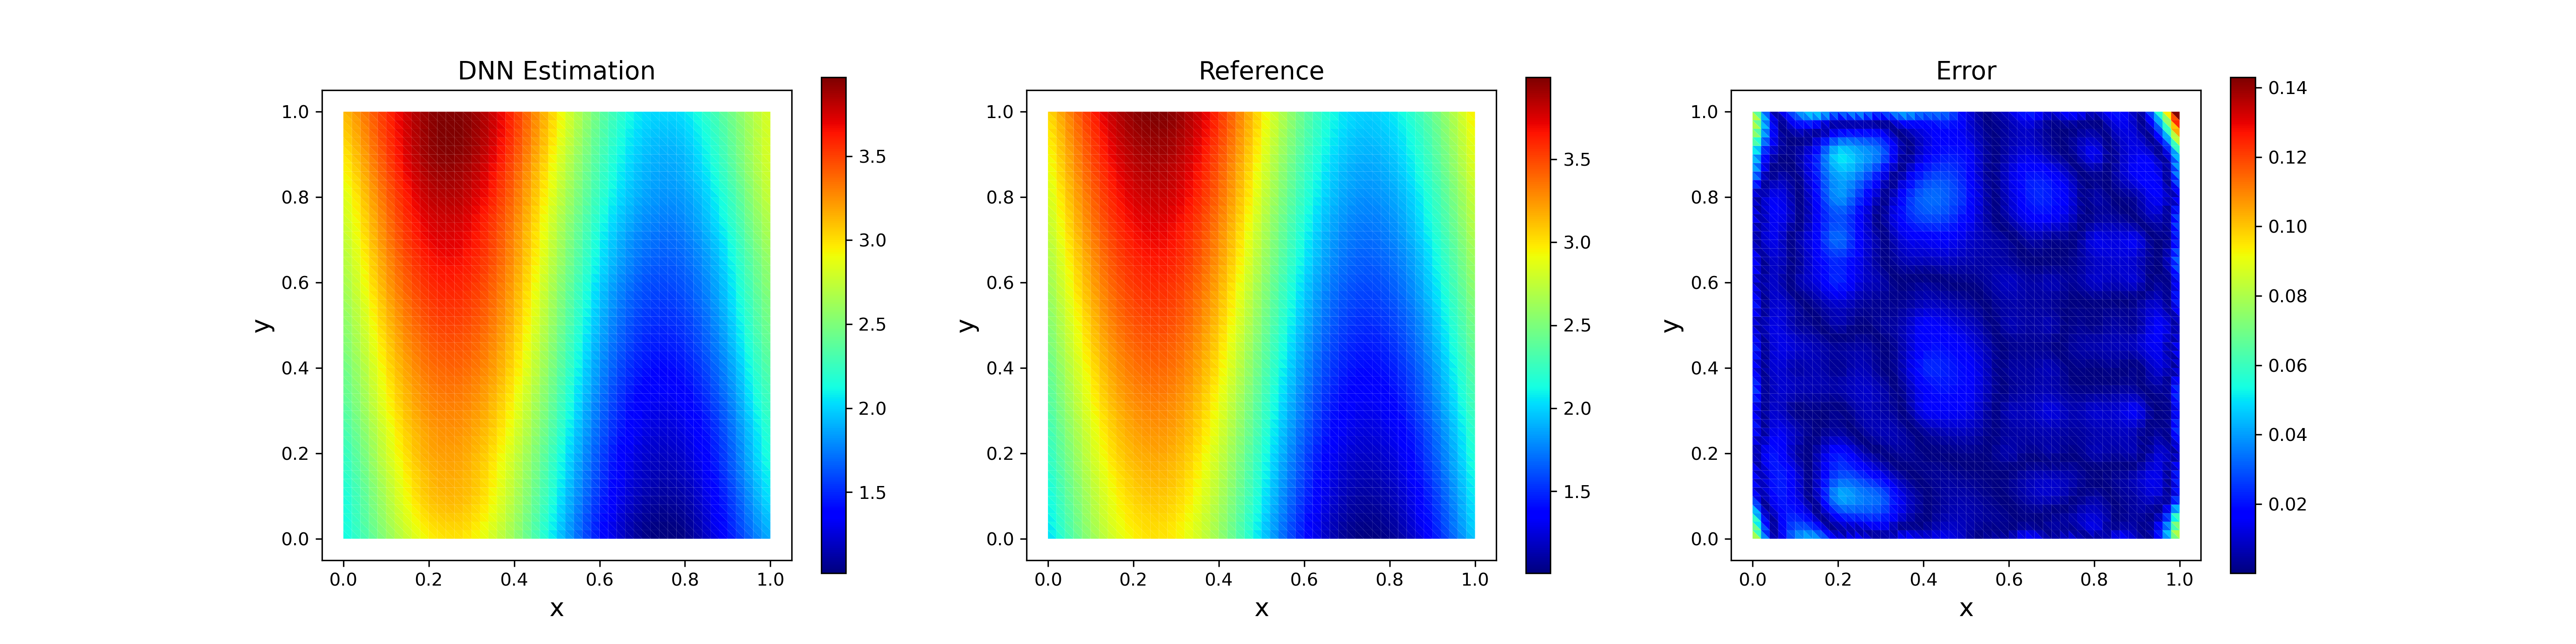
\includegraphics[width=1.0\textwidth]{paper/Kailai/figures/combine_rbf.png}
    \caption{}
    \label{fig:rbf}
\end{figure}

\Cref{fig:closs_nn} shows the loss function trajectory of deep neural networks and radial basis functions. We can see that the deep neural network converge faster and is more accurate. \Cref{fig:nn,fig:rbf} summarize the results for both cases. It is worth noticing that both approaches give good estimations for $\kappa$, but the radial basis function has large error on the right upper corner. This is because in radial basis function approach, there are fewer centroids near the corners.  

\section{Limitations}


\section{Concluding Remarks}

\end{document}
